\documentclass[11pt]{article}
\usepackage{fullpage}
\usepackage{amsfonts}
\usepackage{amssymb}
\usepackage{amsmath}
\usepackage{xcolor}
\usepackage{algorithm}
\usepackage{algorithmic}
\usepackage{enumitem}
\usepackage{fourier}
\usepackage[normalem]{ulem}
\usepackage{graphicx}

\newcommand{\F}{\mathbb{F}}
\newcommand{\np}{\mathop{\rm NP}}
%\newcommand{\binom}[2]{{#1 \choose #2}}

\newcommand{\mnote}[1]{{\color{red} [Madhu: #1]}}
\newcommand{\achnote}[1]{{\color{orange} [Sitan: #1]}}

\newcommand{\Z}{{\mathbb Z}}
\newcommand{\vol}{\mathop{\rm Vol}}
\newcommand{\conp}{\mathop{\rm co-NP}}
\newcommand{\atisp}{\mathop{\rm ATISP}}
\renewcommand{\vec}[1]{{\mathbf #1}}
\newcommand{\cupdot}{\mathbin{\mathaccent\cdot\cup}}
\newcommand{\mmod}[1]{\ (\mathrm{mod}\ #1)}

\setlength{\parskip}{\medskipamount}
\setlength{\parindent}{0in}

\begin{document}

%{\color{brown} Changes after test solvers started looking indicated in brown.}

%{\color{red} Changes after release indicated in red.}

        \section*{CS 124 Homework 1: Spring 2024}

%{\color{brown}        \sout{\textbf{Your name:}}}

        \textbf{Collaborators: } Office hours

        \textbf{No. of late days used on previous psets: } 0 \\
        \textbf{No. of late days used after including this pset: } 0

Homework is due {\color{blue} Wednesday Jan 31 at 11:59pm ET}. You are allowed up to {\bf twelve} late days, but the number of late days you take on each assignment must be a nonnegative integer at most {\bf two}.

Try to make your answers as clear and concise as possible;
style may count in your grades. Assignments must be submitted in pdf format on Gradescope. If you do assignments by hand, you will need to scan your papers to turn them in.


{\bf Collaboration Policy:} You may collaborate on this (and all problem sets) only with other students currently enrolled in the class, and of course you may talk to the Teaching Staff or use Ed. You may also consult the recommended books for the course and course notes linked from the timetable. You may not use Generative AI or large language models, or search the web for solutions, or post the questions on chat forums. Furthermore, you must follow the "one-hour rule" on collaboration.  You may not write anything that you will submit within one hour of collaborating with other students or using notes from such sources. That is, whatever you submit must first have been in your head alone, or notes produced by you alone, for an hour. Subject to that, you can collaborate with other students, e.g. in brainstorming and thinking through approaches to problem-solving.


For all homework problems where you are asked to give an algorithm, you must prove the correctness
of your algorithm and establish the best upper bound that you can give for the running time. Generally
better running times will get better credit; generally exponential-time algorithms (unless specifically asked
for) will receive no or little credit. You should always write a clear informal description of your algorithm
in English. You may also write pseudocode if you feel your informal explanation requires more precision
and detail, but keep in mind pseudocode does NOT substitute for an explanation. Answers that consist
solely of pseudocode will receive little or no credit. Again, try to make your answers clear and concise.

There is a (short) programming problem on this assignment; you {\bf should \textit{NOT} code} with others on
this problem like you will for the ``major'' programming assignments later in the course. (You may
talk about the problem, as you can for other problems.)


\section*{Problems}

\textbf{Please note that Question 4 will use concepts covered on Monday, 1/29 (as well as in sections). Students are advised not to begin this question until after they learn it in a formal setting.}

\begin{enumerate}[leftmargin=*]


\item In class we saw a simple proof that Euclid's algorithm for $n$-bit integers terminates in $O(n)$ steps. In this problem, you will provide a tighter bound on the constant factor in $O(n)$.

Given positive integers $A, B$ satisfying $A \ge B$, let $(A',B') = (B,A \bmod B)$, denote the result of one step of Euclid's algorithm.

\begin{enumerate}
    \item (\textbf{5 points}) Prove that $A' + B' \le \frac{2}{3}(A + B)$. Conclude that starting from $(A,B)$, Euclid's algorithm terminates after at most $\log_{3/2}(A+B)$ steps.
      \begin{quote}
        \color{purple}
        I'll prove the claim by considering two exhaustive cases relating $A$ and $B$. Assume for simplicity that $A \geq B$ must always be true. If not, Euclid's algorithm will swap them and resume that invariant. 

        \medskip
        Consider when $A \geq 2B$. By the definition above, observe the following: 
        \begin{align*}
            && A' + B' && \text{Initial} && \\
            && = B + A \mod B && \text{Substitute by definitions} && \\
            && \leq B + B \mod B && \text{Because $A \mod B < B$} && \\
            && = 2B && \text{Simplify} && \\
        \end{align*} 

        Similarly, because $A \geq 2B$ by the case assumption, we know $A + B \geq 2B + B = 3B$. Join these into an inequality and simplify:
        \begin{align*}
            && A' + B' \leq 2B \leq 3B \leq A + B && \text{Inequalities determined above} && \\
            && A' + B' \leq 2B \leq \frac{2}{3} \cdot 3B \leq \frac{2}{3}(A + B) && \text{Scale right two terms} && \\
            && A' + B' \leq 2B = 2B \leq \frac{2}{3}(A + B) && \text{Simplify} && \\
            && A' + B' \leq \frac{2}{3}(A + B) && \text{Remove intermediate terms} && \\
        \end{align*} 

        Thus, when $A \geq 2B$, it holds that $A' + B' \le \frac{2}{3}(A + B)$. 

        \medskip
        Next, consider then $A < 2B$. Because $A$ is less than $2B$ from 

      \end{quote}
    \item (\textbf{3 points}) In lieu of $A+B$, consider a more general function $g(A,B) = A + \beta B$ for $\beta > 0$. Let $A = QB+R$, where $R$ is the remainder and $Q$ is the quotient when dividing $A$ by $B$. Give an exact expression for $L' = g(A',B')$ solely in terms of $B,R,\beta$, and give a lower bound $L$ for $g(A,B)$ solely in terms of $B, R, \beta$. Briefly justify your answer
    \item (\textbf{5 points}) Define a choice of $\beta$ for which the ratio $L'/L$ in the previous question is always the same regardless of $B,R$. Prove your answer. (Note: $\beta$ and this ratio will be irrational numbers)
    \item (\textbf{5 points}) Use this choice of $\beta$ to prove an improved upper bound on the number of steps of Euclid's algorithm starting from $(A,B)$.
    \item (\textbf{2 points}) Construct an increasing sequence of inputs $(A,B)$ for which the bound in the previous question is asymptotically tight. Informally justify why the sequence you constructed is tight in 1-2 sentences.
\end{enumerate}
(Note; Part (e) above may be attempted independently before attempting other parts and the answer may give a hint to solving Parts (b)-(d).)
% to \emph{polynomials}. Let $\mathbb{Q}[x]$ denote the set of polynomials in the variable $x$ whose coefficients are rational numbers (e.g. $\frac{3}{7}x^3 - 2x + \frac{5}{3} \in \mathbb{Q}[x]$).


\item
On a platform of your choice, implement the three different methods for computing the Fibonacci
numbers (recursive, iterative, and matrix) discussed in lecture. Use integer variables. (You do not need to submit your source code with your assignment.)
\begin{enumerate}
\item
{\bf (15 points)}
How fast does
each method appear to be? (This is deliberately open-ended; part of the problem is to decide what constitutes a reasonable answer.)
Include precise timings if possible---you will need to figure out how to time processes on the system
you are using, if you do not already know.
\begin{quote}
  \color{purple}
  I ran the three algorithms in release-mode Rust using $v1.75.0$ on an M1 Macbook Pro. The recursive and matrix algorithms are identical to the lecture notes. I modified the iterative algorithm to just keep a pointer to the previous two numbers to avoid all the unnecessary heap allocations in a vector. So, it might be a bit faster than otherwise. All three algorithms were tested against each-other for correctness in the range $n = 1$ to $n = 20$. 

  \medskip
  My benchmark was essentially this:
  \begin{algorithm}
  \caption{Test fib}
  \begin{algorithmic}
  \FOR{16 seconds}
      \FOR{n = 1}
          \STATE fibonacci(n)
          \STATE n += 1
      \ENDFOR
  \ENDFOR
  \end{algorithmic}
  \end{algorithm}

  It's a race to see how high of $n$ can be reached in less than 16 seconds (the last run that went over was not counted). After three passes, these were my average results:
  \begin{itemize}
    \item Recursive: n = 47
    \item Iterative: n = 225,248
    \item Matrix: n = 196,768,930
  \end{itemize}

  Based on these benchmarks, the matrix method appears much faster. 
  
  \medskip
  Edit: After seeing part $c$, I realize my test might not look very creative. If you'd like actual times, computing the $32$nd Fibonacci number takes the following times:
  \begin{itemize}
    \item Recursive: 15.812041ms
    \item Iterative: 167ns
    \item Matrix: 83ns
  \end{itemize}

  \medskip
  Edit 2: Part $c$ also required writing my own matrix exponentiation (to accomodate the modding). My own multiplication uses basic $n^3$ multiplication and doesn't use SIMD or any serious optimizations, so I was curious to see how different it was from the graphics library. Here are the new results (Edit 3: these were found before I added timeouts mentioned in part $c$): 
  \begin{itemize}
    \item Recursive: n = 47
    \item Iterative: n = 202,663
    \item Matrix (my implementation): n = 55,309,376
    \item Matrix (nalgebra crate): n = 198,068,230
  \end{itemize}

  \medskip
  And new times. My matrix implementation and iterative are the same here, but the difference is at the nanosecond level, so asymptotic behavior is much more effectively approximated by the 16 second tests.
  \begin{itemize}
    \item Recursive: 15.025ms
    \item Iterative: 125ns
    \item Matrix (my implementation): n = 125ns
    \item Matrix (nalgebra crate): n = 83ns
  \end{itemize}
\end{quote}
\item
{\bf (4 points)}
What's the first Fibonacci number that's at least $2^{31}$? (If you're using C longs, this is where you hit
integer overflow.)
\item
  \begin{quote}
    \color{purple}
  The \textbf{47th} Fibonacci number is $2,971,215,073$, which exceeds $2^{31} = 2,147,483,648$. 
  \end{quote}
{\bf (15 points)}
Since you should reach ``integer overflow'' with the faster methods quite quickly, modify your programs
so that they return the Fibonacci numbers modulo $2^{16}$. (In other words, make all of your
arithmetic modulo $2^{16}$---this will avoid overflow! You must do this regardless of whether or not your
system overflows.) For each method, what is the largest value of $k$ such that you can compute the
$k^\text{th}$ Fibonacci number (modulo 65536) in one minute of machine time? If that value of $k$ would be too big to handle (e.g. if you'd get integer overflow on $k$ itself) but you can still calculate $F_{k}$ quickly, you may report the largest value $k_{max}$ of $k$ you can handle and the amount of time the calculation of $F_{\rm k_{max}}$ takes. 
\begin{quote}
  \color{purple}
  I changed my code substantially this problem. Now, the algorithms perform modulo arithmetic on intermediate Fibonacci numbers, and they carry timers so that long-running functions can interrupt themselves. Polling the timers seems to meaningfully slow down each recursive frame and iterative pass. I also wrote my own matrix exponentiation (instead of the graphics library from part $a$), and I added a function that binary-searches for the input to an algorithm that halts than 60 seconds with correct output. 

  \medskip
  My matrix exponentiation algorithm calculates the (mod $2^16$) Fibonacci number for Rust's $u64::MAX = 18446744073709551615$ value in much less than a second. This surprised me a lot. I wrote a test to ensure recursive, iterative, and matrix all produce the same values up to the 20th Fibonacci number and a similar test for just matrix and iterative up to the $2^12$th Fibonacci number. I really don't think my matrix implementation is incorrect. Because exponentiation is essentially $\lg n$ and $\lg 2^{64} = 64$, my conclusion is that computing the maximum non-overflow Fibonacci number on my computer in microseconds when a low Fibonacci number takes nanoseconds might make sense.

  \begin{itemize}
    \item Recursive: Computed $k = 45$ in less than one minute. (This is slower than the 16 seconds test from $a$, but checking the timer at every frame had a big impact)
    \item Iterative: Computed $k = 2,464,538,623$ in less than one minute.
    \item Matrix: Computed $k = 18446744073709551615$ (maximum unsigned 64-bit integer) in $1.208$ microseconds.
  \end{itemize}

\end{quote}
\end{enumerate}


\item
\begin{enumerate}
\item
{\bf (10 points)}
Make all true statements of the form $f_i \in o(f_j)$, $f_i \in O(f_j)$, $f_i \in \omega(f_j)$, and $f_i \in \Omega(f_j)$ that hold for $i \le j$, where $i, j \in \{1,2,3,4,5\}$ for the following functions. No proof is necessary. All logs are base 2 unless otherwise specified.
\begin{enumerate}
\item $f_1 = (\log n)^{\log n}$
\item $f_2 = 2^{\sqrt{\log n}}$
\item $f_3 = 2^{{\color{red}(}2^{\sqrt[3]{\log\log\log n}}{\color{red})}}$
\item $f_4 = n^{\log\log n}$
\item $f_5 = (\log\log n)^n$
\end{enumerate}
\item
{\bf (5 points)}
Give an example of a function $f_6: \mathbb{N} \to \mathbb{R}^+$ for which \emph{none} of the four statements $f_i \in o(f_6)$, $f_i \in O(f_6)$, $f_i \in \omega(f_6)$, and $f_i \in \Omega(f_6)$ is true for any $i \in \{1,2,3,4,5\}$.
\end{enumerate}

\item \begin{enumerate}
    \item Solve the following recurrences exactly, and then prove your solutions are correct:
    (Hint: Calculate values and guess the form of a solution. Then prove that your guess is correct by induction.)
    \begin{enumerate}
        \item
        {\bf (5 points)} 
        $T(1) = 1$, $T(n) = T(n-1) + n^2 - n$
        \begin{quote}
          \color{purple}
          \medskip
          \textit{Derivation}: \\
          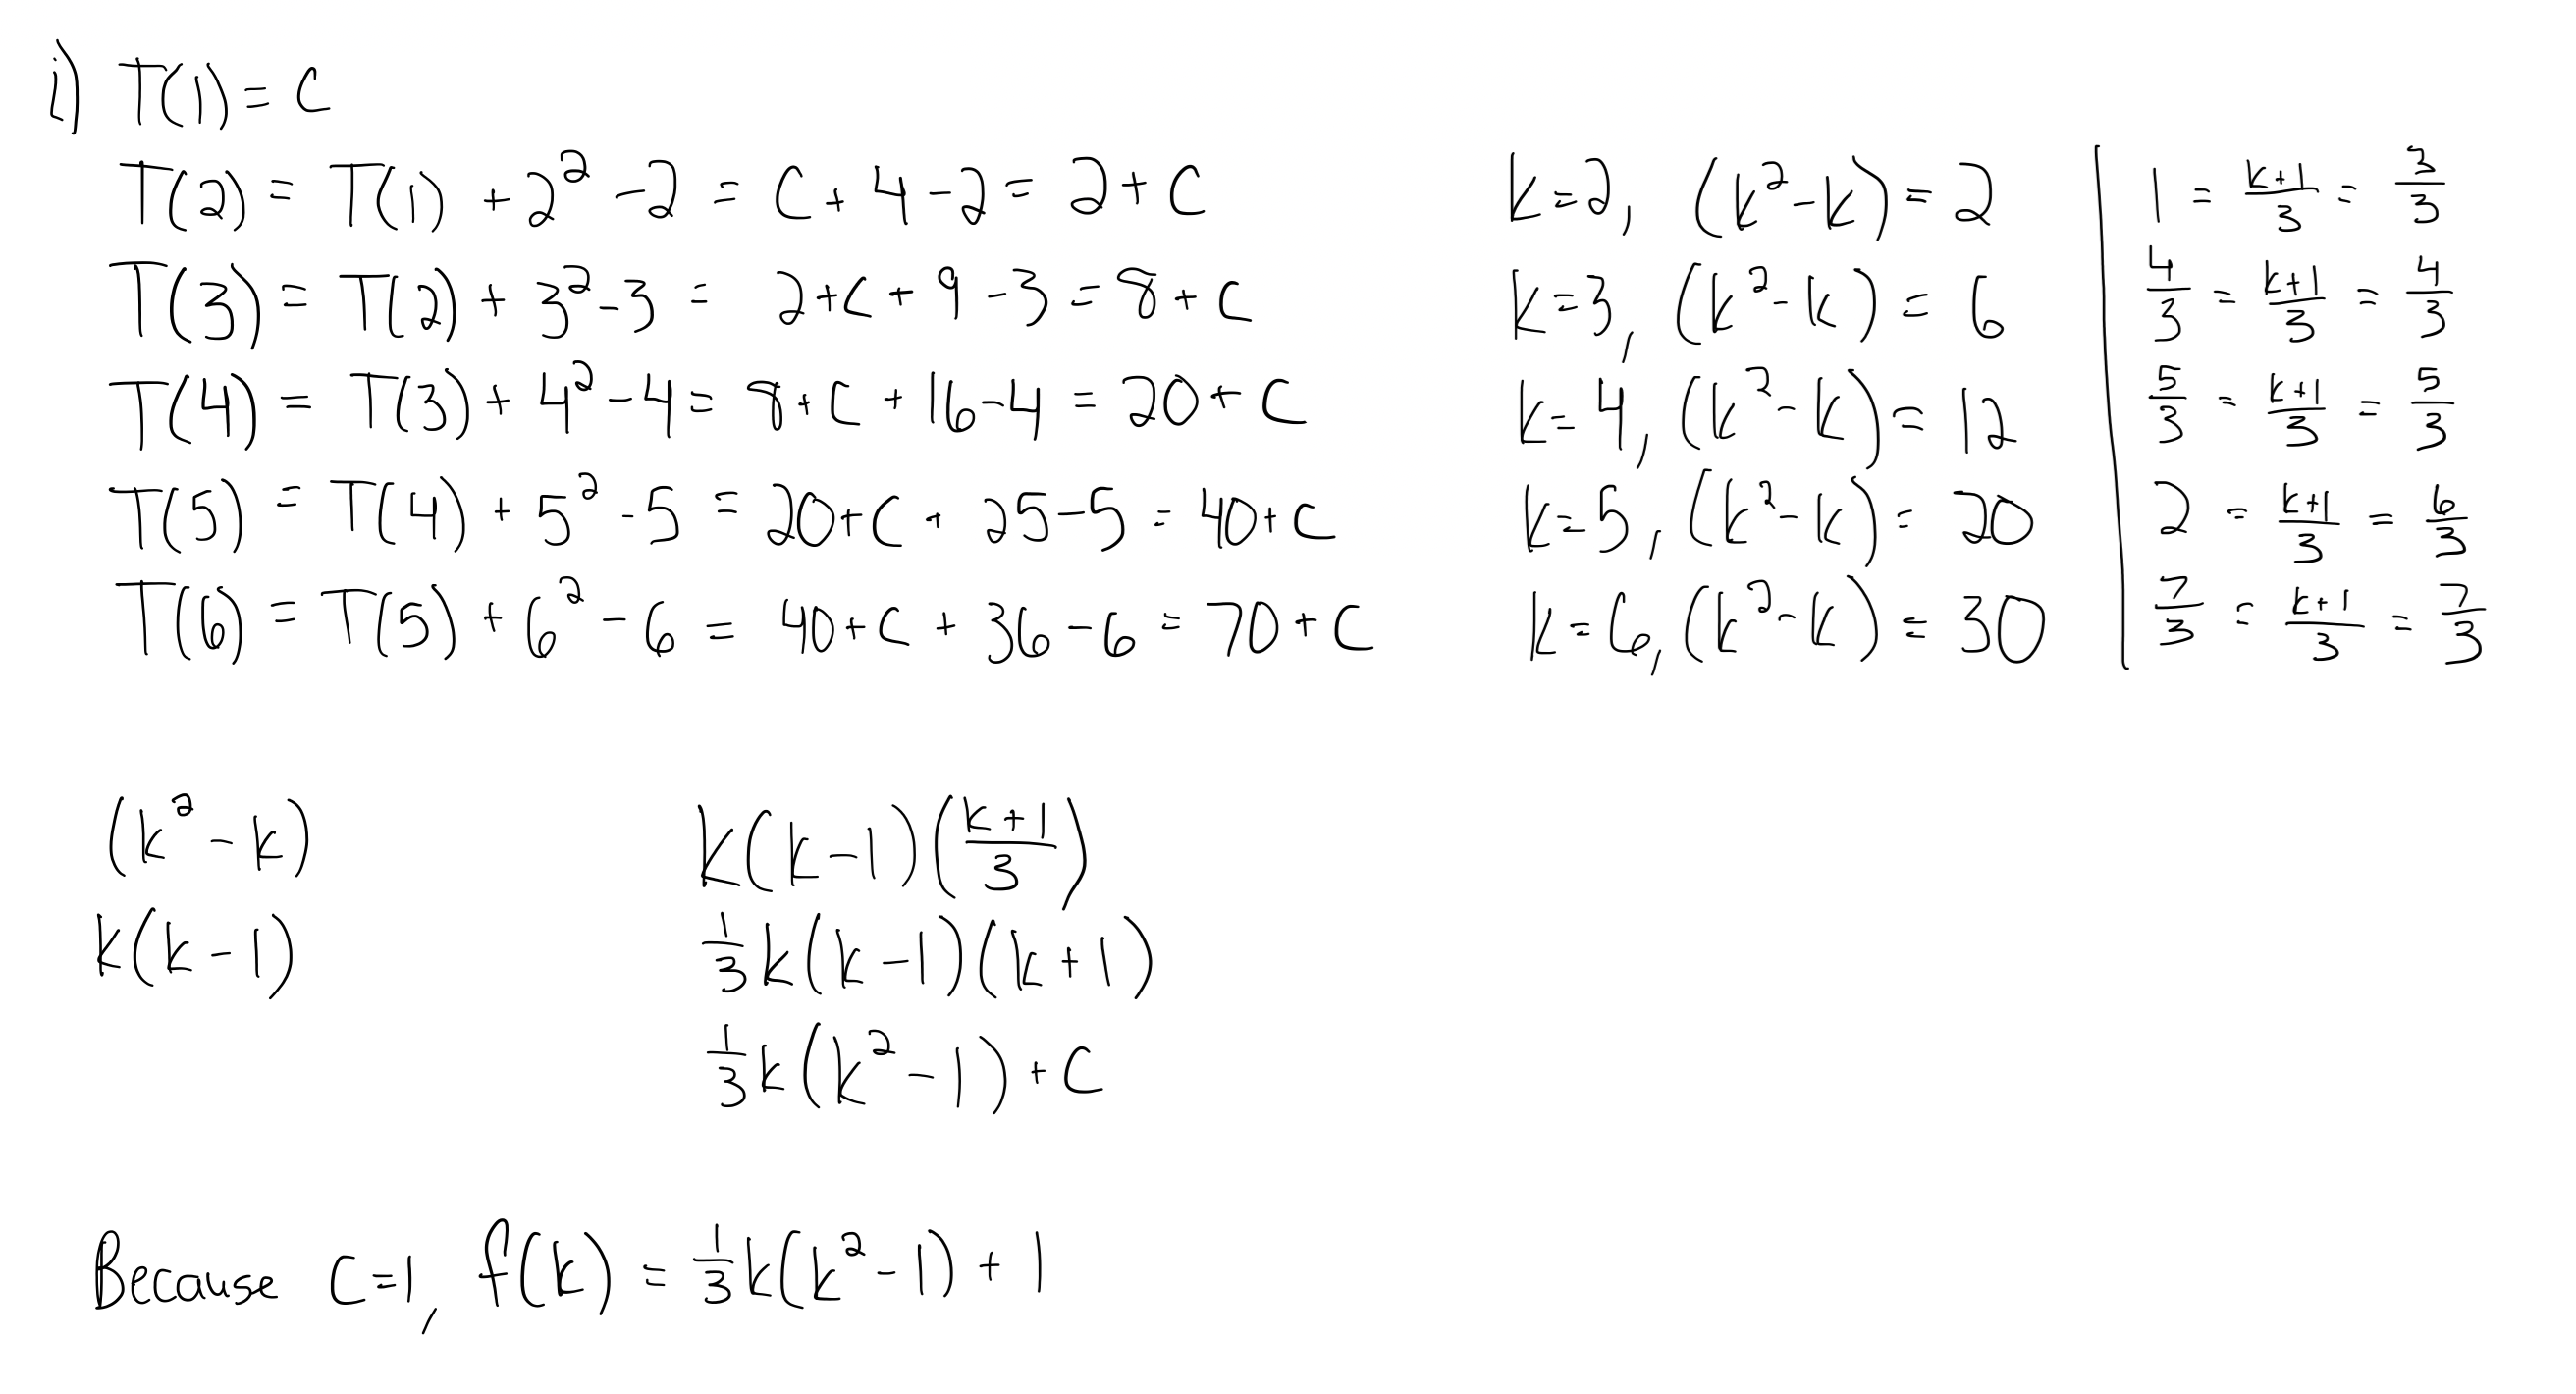
\includegraphics[width=0.8\linewidth]{"./pics/4ai.png"}

          \medskip
          Claim: the closed form is $f(n) = \frac{1}{3}n(n^2 - 1) + 1$.

          \medskip
          Proof by induction on $n$: \\ 
          \textit{Base case}: For $n = 1$, $T(1) = 1$ is given by the definition, and $f(1) = \frac{1}{3}(1)(1^2 - 1) + 1 = 1$. So, the base case holds.

          \medskip
          \textit{Inductive hypothesis}: Assume the claim is true for all $k$ from $1 \leq k \leq n$.

          \medskip
          \textit{Inductive step}: Consider $T(n + 1)$:
          \begin{align*}
              && T(n + 1) = T(n + 1 - 1) + (n + 1)^2 - (n - 1) && \text{Initial} && \\
              && = T(n) + n^2 + n && \text{Simplify} && \\
              && = \frac{1}{3}n(n^2 - 1) + 1 + n^2 + n && \text{Apply inductive hypothesis} && \\
              && = \frac{1}{3}n^3 + n^2 + \frac{2}{3}n + 1 && \text{Simplify} && \\
          \end{align*} 

          \medskip
          Similarly, consider $f(n + 1)$:
          \begin{align*}
              && f(n + 1) = \frac{1}{3}(n + 1)((n + 1)^2 - 1) + 1 && \text{Initial} && \\
              && = (\frac{1}{3}n + \frac{1}{3})(n^2 + 2n) + 1 && \text{Distribute and FOIL} && \\
              && = \frac{1}{3}n^3 + n^2 + \frac{2}{3}n + 1 && \text{Multiply and combine} && \\
          \end{align*} 

          \medskip
          Thus, $T(n + 1) = f(n + 1)$, proving the inductive step. By induction, the closed form of the recurrence must be correct. 
        \end{quote}
        \item
        {\bf (5 points)}
        $T(1) = 1$, $T(n) = 3T(n-1) - n + 1$
        \begin{quote}
          \color{purple}
          Derivation: \\ 
          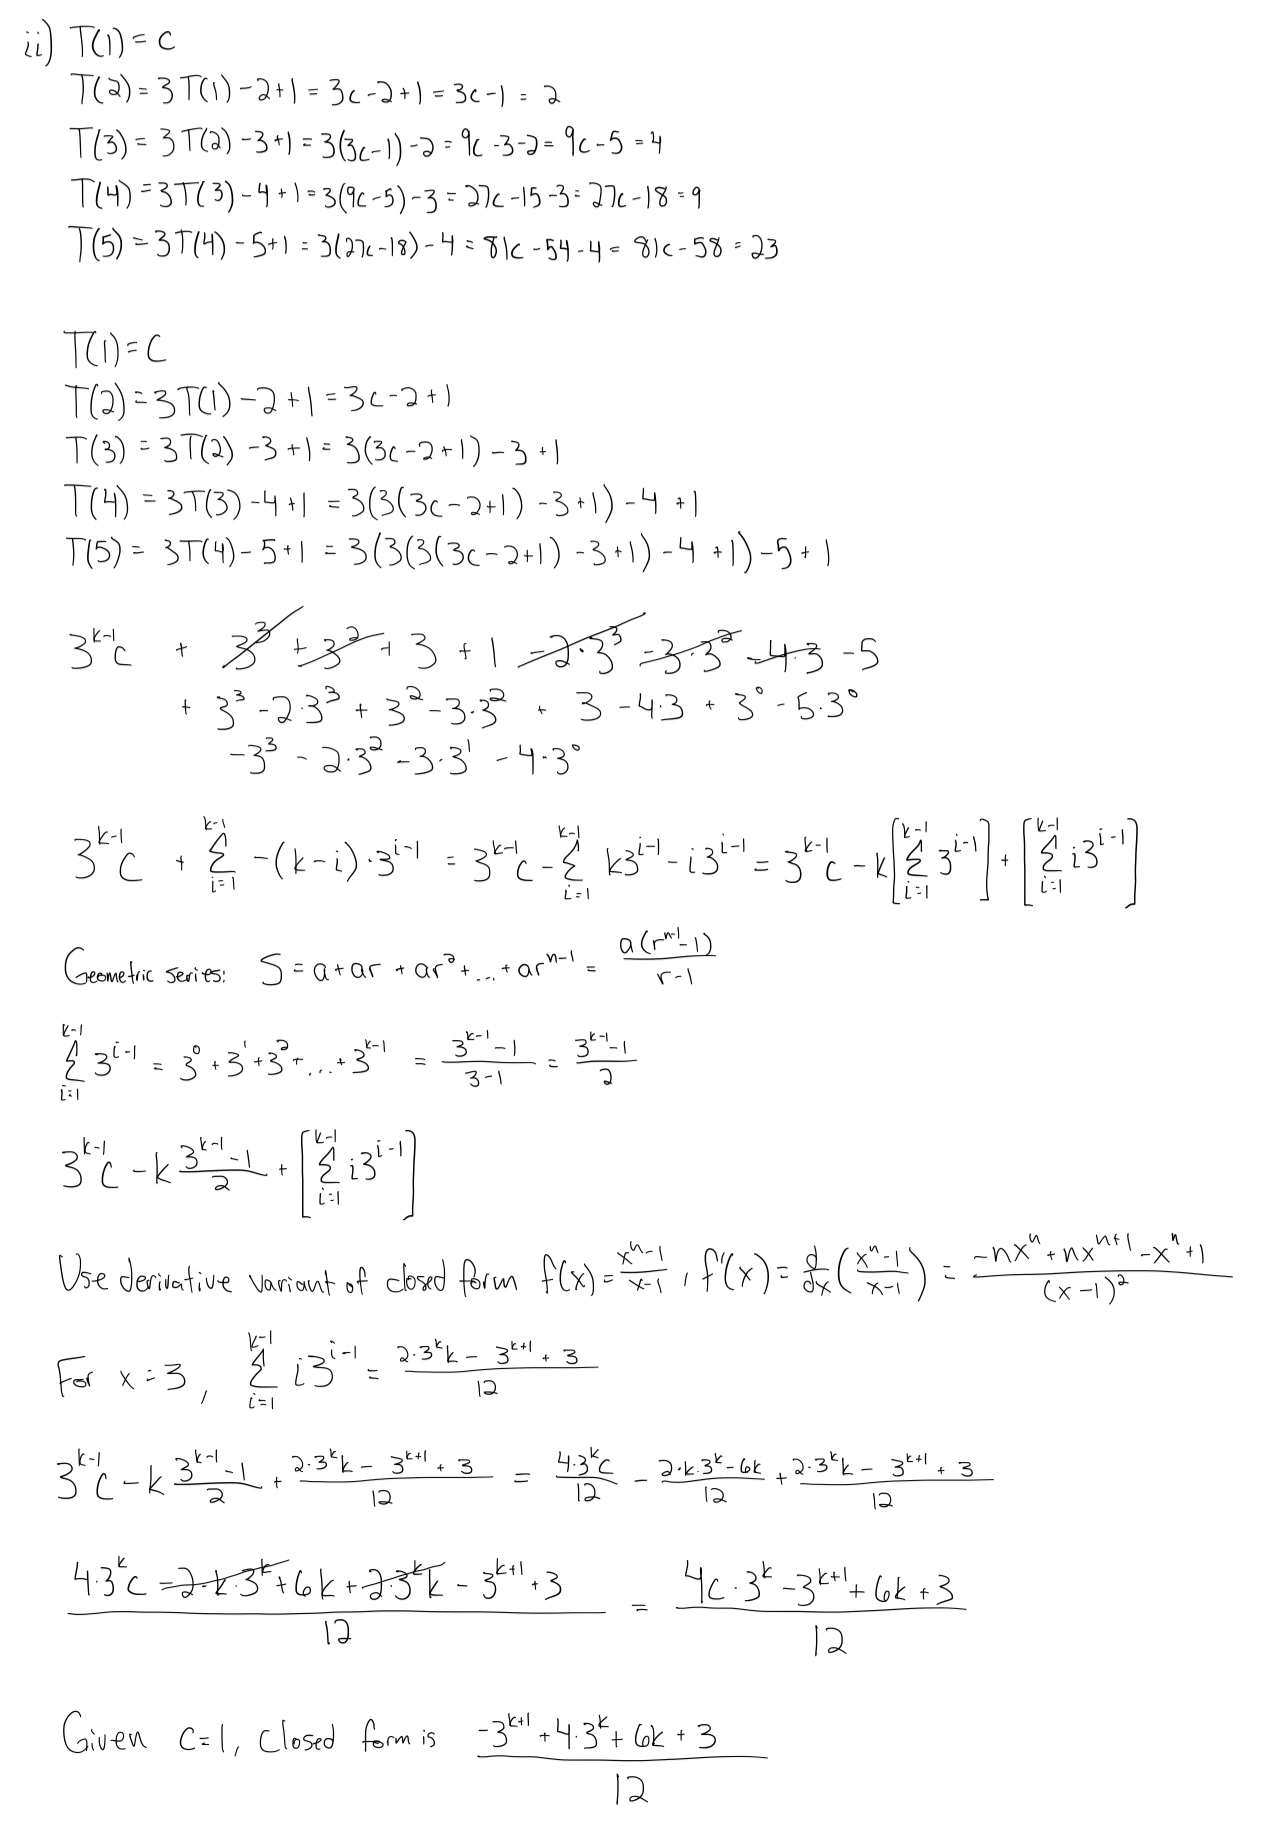
\includegraphics[width=0.8\linewidth]{"./pics/4aii.png"}

          \medskip
          Claim: the closed form is $f(n) = \frac{-3^{n + 1} + 4 \cdot 3^n + 6n + 3}{12}$.


          \medskip
          Proof by induction on $n$: \\ 
          \textit{Base case}: For $n = 1$, $T(1) = 1$ is given by the definition, and $f(1) = \frac{-3^2 + 4 \cdot 3 + 6 + 3}{12} = \frac{-9 + 21}{12} = 1$. So, the base case holds.

          \medskip
          \textit{Inductive hypothesis}: Assume the claim is true for all $k$ from $1 \leq k \leq n$.

          \medskip 
          \textit{Inductive step}: Consider $T(n + 1)$: 
          \begin{align*}
              && T(n + 1) = 3T(n + 1 - 1) - (n + 1) + 1 && \text{Initial} && \\
              && = 3T(n) - n && \text{Simplify} && \\
              && = 3 \cdot \frac{-3^{n + 1} + 4 \cdot 3^n + 6n + 3}{12} - n && \text{Apply inductive hypothesis} && \\
              && = \frac{-3 \cdot 3^{n + 1} + 4 \cdot 3 \cdot 3^n + 18n + 9 - 12n}{12} && \text{Distribute, join terms} && \\
              && = \frac{-3^{n + 2} + 4 \cdot 3^{n + 1} + 6n + 9}{12} && \text{Merge $3$s into exponents} && \\
          \end{align*} 

          \medskip 
          Similarly, consider $f(n + 1)$:
          \begin{align*}
              && f(n + 1) = \frac{-3^{n + 2} + 4 \cdot 3^{n + 1} + 6(n + 1) + 3}{12} && \text{Initial} && \\
              && = \frac{-3^{n + 2} + 4 \cdot 3^{n + 1} + 6n + 9}{12} && \text{Distribute} && \\
          \end{align*} 

          \medskip
          Thus, $T(n + 1) = f(n + 1)$, proving the inductive step. By induction, the closed form of the recurrence must be correct. 
        \end{quote}
    \end{enumerate}
    \item Give tight asymptotic bounds for $T(n)$ (i.e. $T(n) = \Theta(f(n))$ for some $f$) in each of the following recurrences:
    \begin{enumerate}
        \item
        {\bf (3 points)}
        $T(n) = 9T(\lfloor n/3 \rfloor) + n^2 + 3n$
        \begin{quote}
          \color{purple}
          $T(n) = \Theta(n^2 \cdot \lg n)$

          \medskip
          Proof by case II of the Master Theorem where $a = 9$, $b = 3$, and $f(n) = n^2 + 3n$:

          \medskip
          $O(n^{log_{3}9} \cdot (\lg n)^k)$ where $k = 0$ simplifies to $O(n^2)$. Because $f(n) = n^2 + 3n = O(n^2)$, the upper bound in the second case of the Master Theorem is satisfied.

          \medskip
          $\Omega(n^{log_{3}9} \cdot (\lg n)^k)$ similarly simplifies to $\Omega(n^2)$ when $k = 0$. Because $f(n) = n^2 + 3n = \Omega(n^2)$, the lower bound in the second case of the Master Theorem is satisfied.

          Assert from $CLRS$ page $102$ that the asymptotic bounds provided by the Master Theorem are not affected by floor or ceiling rounding, so this bound also applies to the given equation.

          \medskip
          Thus, by the second case of the Master Theorem, assert that $T(n) = \Theta(n^{\log_{3}9} \cdot (\lg n)^{1})$, which simplifies to $T(n) = \Theta(n^2 \cdot \lg n)$.
        \end{quote}
        \item 
        {\bf (7 points)}
        $T(n) = 4T(\lfloor \sqrt{n} \rfloor) + \log n$ (Hint: it may help to apply a change of variable)
        \begin{quote}
          \color{purple}
          $T(n) = \Theta((\lg n)^2)$

          \medskip
          Because proving this bound requires a change of variable, my analysis determines an upper bound (and the bound itself) using the Master Theorem and proves the lower bound using substitution. 

          \medskip
          In both parts, let $k = \lg n$.
          
          \medskip 
          \textbf{Upper bound}:
          Let $t$ be $T$ without any floor function. Due to the floor function, a complete upper bound on this recurrence is $t(n) = 4t(\sqrt n) + \lg n$. Because $2^k = n$, let $t(2^k) = 4t(\sqrt{2^k}) + \lg{2^k} = 4t(2^{\frac{1}{2}k}) + k$.

          \medskip
           Let $R(k) = t(2^k)$. By this definition, $R(\lg n) = t(2^{\lg n}) = t(n)$. Similarly, $R(k) = 4R(\frac{1}{2}k) + k$.

          \medskip
          Consider case I of the Master Theorem on $R(k)$ where $a = 4$, $b = 2$, $f(k) = k$, and $\lg 4 = 2$. Because $f(k) = k = O(k^{2 - \epsilon})$ where $\epsilon \leq 1$, the case is satisfied and the Master Theorem asserts that $R(k) = \Theta(k^2)$.

          \medskip
          De-substituting this yields the following:
          \begin{itemize}
            \item $R(k) = \Theta(k^2)$ 
            \item $R(\lg n) = \Theta((\lg n)^2)$
            \item $T(n) = \Theta((\lg n)^2)$
          \end{itemize}

          Thus, by the Master Theorem and substitutions above, assert that the upper bound on $T(n)$ indicated is $O((\lg n)^2)$. 

          \medskip
          \textbf{Lower bound}:
          Let $R(k) = T(2^k)$. Using the same definition of $k$, we have $T(n) = 4T(\lfloor \sqrt{n} \rfloor) + \log n$ and $T(k) = 4T(\lfloor 2^{\frac{1}{2}k} \rfloor) + k$. This yields $R(k) = 4R(\lg(\lfloor 2^{\frac{1}{2}k} \rfloor)) + k$.

          \medskip
          Assert that $\frac{k}{2} - 1 \leq \lg(\lfloor 2^{\frac{1}{2}k} \rfloor)$ for all $k > 0$. 

          \medskip
          Under that assertion, $R(k) = 4R(\lg(\lfloor 2^{\frac{1}{2}k} \rfloor)) + k \geq H(k)$ where $H(k) = 4R(\frac{k}{2} - 1) + k$ for all $k > 0$. 

        \medskip
      I'll then prove by substitution that $H(k) = \Omega(k^2)$ for all $k$. Definition of $\Omega$ specifies that $H(k)$ must be greater than $c \cdot k^2$ for $c > 0$ and sufficiently large $k_0 \leq k$. Here, let $c = 0.1$ and $k_0 = 1$. Prove by induction on $k$: 

        \medskip
        \textit{Base case}: At $k = 0$, $H(1) = 4 \cdot H(\frac{1}{2} - 1) + 1 \geq 0.1(1^2) = 0.1$, assuming the output of $H$ is always nonnegative.

        \medskip
        \textit{Inductive hypothesis}: Assume that $ck^2 \leq H(k)$ for all $k_0 \leq k$. 

        \medskip
        \textit{Inductive step}: Consider the following.
        \begin{align*}
            && H(k + 1) = 4H(\frac{k + 1}{2} - 1) + k + 1 && \text{Initial} && \\
            && = 4H(\frac{1}{2}k - \frac{1}{2}) + k + 1 && \text{Simplify fraction} && \\
            && \geq 4c \cdot (\frac{1}{2}k - \frac{1}{2})^2 + k + 1 && \text{By inductive hypothesis} && \\
            && = 4c \cdot (\frac{1}{4}k^2 - \frac{1}{2}k + \frac{1}{4}) + k + 1 && \text{FOIL} && \\
            && = ck^2 - 2ck + c + k + 1 && \text{Distribute} && \\
            && = 0.1k^2 + 0.8k + 1.1 && \text{Substitute $c = 0.1$} && \\
            && \geq c(k + 1)^2 && \text{Greater than assumed bound} && \\
            && = 0.1k^2 + 0.2k + 0.1 && \text{Expanded for clarity} && \\
        \end{align*} 

        Because $c(k + 1)^2 \leq H(k + 1)$, the claim holds by induction. This proves that $H(k) = \Omega(k^2)$. Because $H(k) \leq R(k)$ for all $k \geq 1$, it must also hold that $R(k) = \Omega(k^2)$. Substituting in terms of $n$ yields $R(\lg n) = \Omega((\lg n)^2)$. Finally, substituting functions produces $T(n) = \Omega((\lg n)^2)$. 


        \medskip
        \textbf{Conclusion}:
        The two cases above prove that the recurrence $T(n)$ is both $O((\lg n)^2)$ and $\Omega((\lg n)^2)$, proving that $T(n) = \Theta((\lg n)^2)$.
        \end{quote}
    \end{enumerate}
\end{enumerate}

\item One of the simplest algorithms for sorting is BubbleSort --- see code below.

\begin{algorithm}
\caption{BubbleSort}
\begin{algorithmic}
\STATE Input: $A[0], \dots, A[n-1]$
\FOR{$i = 0$ to $n - 1$}
    \FOR{$j = 0$ to $n - 2$}
        \IF{$A[j] > A[j+1]$}
            \STATE Swap $A[j]$ and $A[j+1]$
        \ENDIF
    \ENDFOR
\ENDFOR
\end{algorithmic}
\end{algorithm}

In this problem we will study the behavior of a twisted version of BubbleSort, described below.

\begin{algorithm}
\caption{TwistedBubbleSort}
\begin{algorithmic}
\STATE Input: $A[0], \dots, A[n-1]$
\FOR{$i = 0$ to $n - 1$}
    \FOR{$j = 0$ to $n - 1$}
        \IF{$A[i] < A[j]$}
            \STATE Swap $A[i]$ and $A[j]$
        \ENDIF
    \ENDFOR
\ENDFOR
\end{algorithmic}
\end{algorithm}

Your task is to prove that TwistedBubbleSort also correctly sorts every array. (While not necessary, you may assume for simplicity that the elements of $A$ are all distinct.)

\begin{enumerate}
    \item (\textbf{2 points}) Explain in plain English why TwistedBubbleSort is different from BubbleSort. I.e., describe at least one difference in the swaps made by the two algorithms.
      \begin{quote}
        \color{purple}
        Bubble sort operates by comparing and swapping neighbors. The upper index $i$ exists to ensure enough such comparisons are made. In contrast, TwistedBubbleSort chooses an index $i$ for a cycle of iteration and compares all numbers in the array to the value currently at $i$. At iteration $i$, it only performs swaps involving $i$, unlike BubbleSort, which performs operations on $j$ and $j$'s neighbor.
      \end{quote}
    \item (\textbf{5 points}) Prove that after the $i$-th iteration of the outer loop of TwistedBubbleSort, the largest element of $A$ is at the $i$-th index.
      \begin{quote}
        \color{purple}
        Let $i$ be any valid index in the array. The proof below uses induction on $j$ to prove that, after the inner $j$-loop completes, the largest element of $A$ is in $A[i]$. Assume for simplicity that all elements are distinct and that the syntax $A[m..=n]$ denotes an inclusive subarray. 

        \medskip
        Below is a proof that after finishing step $j$, $0 \leq j \leq n - 1$ of the $j$-loop, the value at $A[i]$ is greater than every value in $A[0..=j]$ excluding $A[i]$.

        \medskip
        \textit{Base case}: $j = 0$. If $A[i] < A[0]$, the value at $A[0]$ is swapped into $A[i]$. This results in $A[i]$ being greater than every element in $A[0..=0]$ excluding $A[i]$. 

        \medskip
        \textit{Inductive hypothesis}: After completing step $j \geq 0$, assume the value at $A[i]$ is greater than all elements from $A[0..=j]$ excluding $A[i]$. 

        \medskip 
        \textit{Inductive step}: Consider step $j + 1$ by cases. 
        \begin{itemize}
          \item If $A[j + 1] = A[i]$ (by the simplification assumption, only true if $i = j + 1$), then the algorithm performs a trivial swap and, by the inductive hypothesis, the subarray $A[0..=j+1]$ excluding $A[i]$ still has no elements greater than $A[i]$. 
          \item If $A[j + 1] < A[i]$, then the subarray is now one element larger. By the inductive hypothesis, there are no elements in $A[0..=j]$ excluding $A[i]$ greater than $A[i]$, and the element at $A[j + 1]$ is also not greater than $A[i]$. Thus, every element in the expanded subarray $A[0..=j + 1]$ excluding $A[i]$ is still less than $A[i]$. 
          \item If $A[j + 1] > A[i]$, then the elements at index $j + 1$ and $i$ are swapped. After they're swapped, $A[j + 1] < A[i]$, and the case above now applies. 
        \end{itemize}

        Across all three cases, after step $j + 1$, the value at $A[i]$ is still greater than every element in the subarray $A[0..=j + 1]$ excluding $A[i]$. This proves the claim true by induction. 

        \medskip
        By the inductive proof above, for any index $i$, after iteration $j = n - 1$, it must be true that the value at $A[i]$ is greater than every element in the (sub)array $A[0..=n-1]$, which is equivalent to saying the largest element of $A$ is at index $i$.
      \end{quote}
    \item (\textbf{10 points}) Prove that after the $i$-th iteration of the outer loop of TwistedBubbleSort, indices $0$ to $i$ of the array are sorted.
      \begin{quote}
        \color{purple}
        Below is a proof by induction on $i$ that the subarray $A[0..=i]$ is in sorted order after the $i$th iteration of the outer loop in TwistedBubbleSort. The subarray syntax is defined above, and sorting is least to greatest. I'm again making the simplifying assumption that every element in the array is distinct.

        \medskip
        \textit{Base case}: $i = 0$. Any number in the subarray $A[0..=0]$ is trivially sorted, so the claim is true for $i = 0$.

        \medskip
        \textit{Inductive hypothesis}: At index $0 \leq i \leq n - 1$, the subarray $A[0..=i]$ is sorted from least to greatest.

        \medskip 
        \textit{Inductive step}: At index $i + 1$, consider the inner loop. By the proof above (question 5b), by the end of the $j$-loop, the greatest element in the array is at index $i + 1$. Because $A[0..=i]$ is already in sorted order (inductive hypothesis) and $A[i + 1]$ must be greater than all in $A[0..=i]$,  it must be true that the expanded subarray $A[0..=i + 1]$ is also now also in sorted order.

        \medskip
        By induction, it must then be true that after the $i$th iteration, indices $0$ to $i$ are in sorted order.
      \end{quote}
\end{enumerate}
    

\item
{\bf (0 points, optional)}\footnote{This question will not be used for grades, but try it if you're interested.
It may be used for recommendations or TF hiring.}
InsertionSort is a simple sorting algorithm that works as follows on input $A[0]$, \ldots, $A[n-1]$.
\begin{algorithm}
\caption{InsertionSort}
\begin{algorithmic}
\STATE Input: $A[0], \dots, A[n-1]$
\FOR{$i = 1$ to $n - 1$}
        \STATE{$j = i$}
        \WHILE{$j > 0$ and $A[j - 1] > A[j]$}
                \STATE Swap $A[j]$ and $A[j - 1]$
                \STATE{j = j - 1}
        \ENDWHILE
\ENDFOR
\end{algorithmic}
\end{algorithm}

Show that for every function $T(n) \in \Omega(n) \cap O(n^2)$
there is an infinite sequence of inputs $\{A_k\}_{k=1}^{\infty}$
such that $A_k$ is an array of length $k$, and if $t(n)$ is the running time of
InsertionSort on $A_n$, then $t(n) \in \Theta(T(n))$.


\end{enumerate}

\end{document}
